\begin{tikzpicture}[x={(1cm,0cm)},y={(0cm,1cm)},z={(0.410cm,0.300cm)}]
    \node[canvas is zy plane at x=0,draw,fill=white] (g0) at (0,0) {
    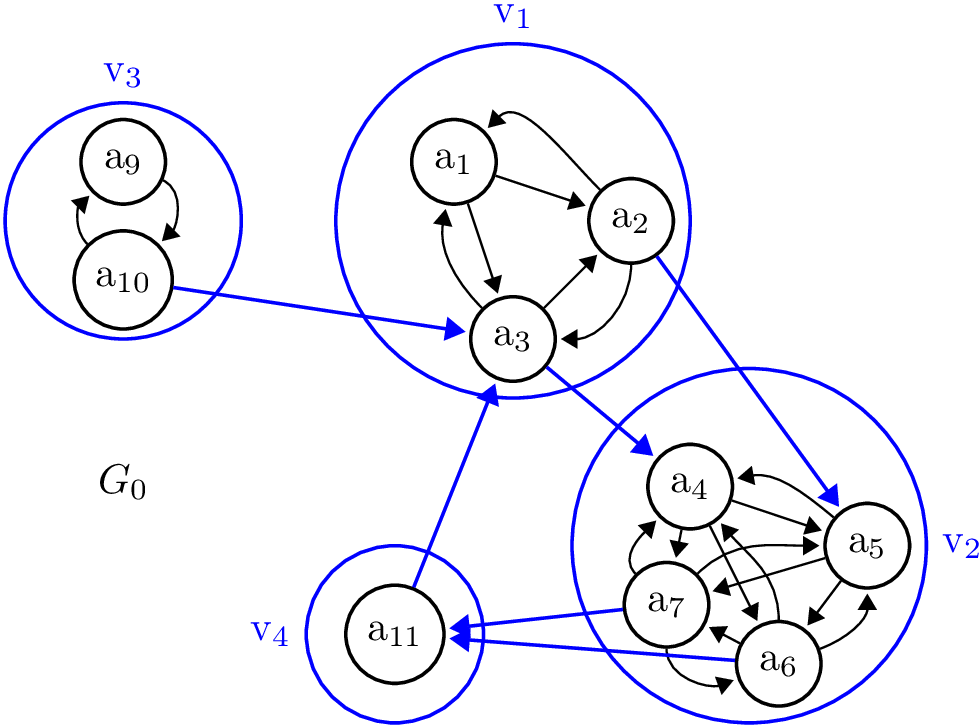
\includegraphics[scale=0.315]{immagini/graph0.png}
    };
    \node[canvas is zy plane at x=5,draw,fill=white] (g1) at (0,0) {
        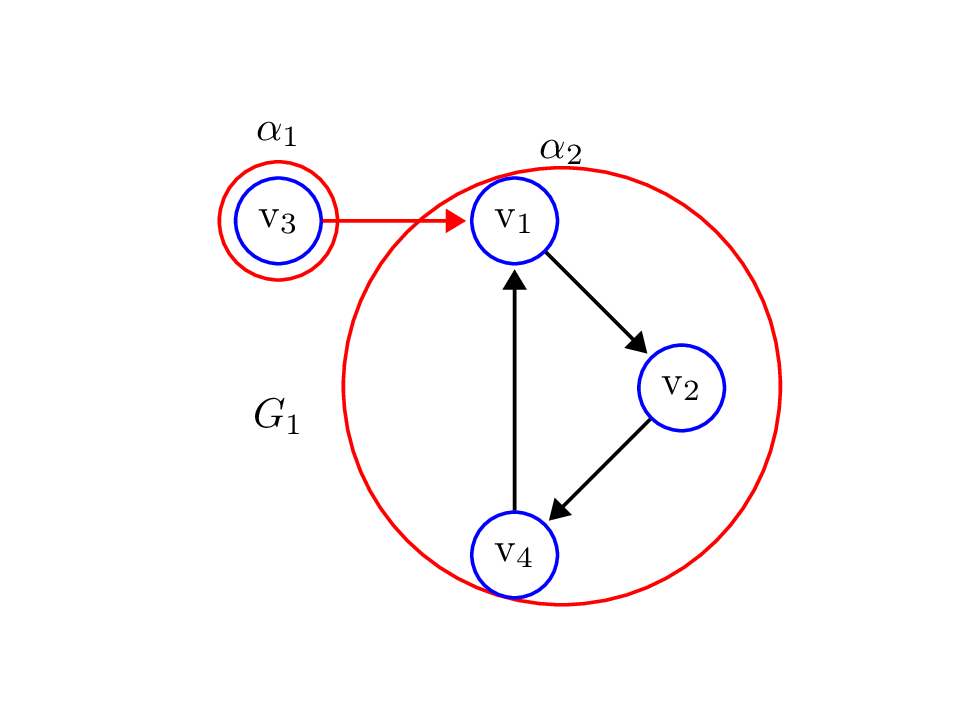
\includegraphics[scale=0.315]{immagini/graph1.png}
    };
    \node[canvas is zy plane at x=10,draw,fill=white] (g2) at (0,0) {
        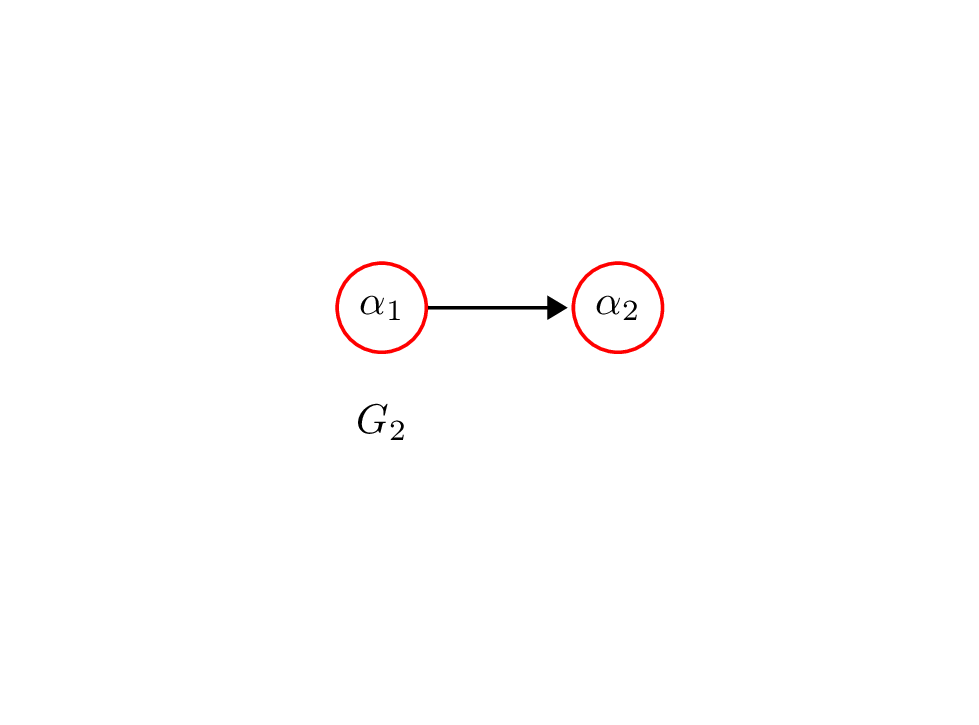
\includegraphics[scale=0.315]{immagini/graph2.png}
    };

    \node (G0) [below of=g0, node distance=5.2cm] {\huge $G_0$};
    \node (G1) [below of=g1, node distance=5.2cm] {\huge $G_1$};
    \node (G2) [below of=g2, node distance=5.2cm] {\huge $G_2$};

    \node (G0d) [below of=G0, node distance=1cm] {};
    \node (G1d) [below of=G1, node distance=1cm] {};
    \node (G2d) [below of=G2, node distance=1cm] {};

    \draw[->, line width=2pt, redUnicam] (G0d) -- (G1d) node[midway, below, red] {\huge $f_{C_1}$};
    \draw[->, line width=2pt, redUnicam] (G1d) -- (G2d) node[midway, below, red] {\huge $f_{C_2}$};
\end{tikzpicture}